Nas seções anteriores, estudamos o pareamento no caso mais simples possível: quando a comparação entre tratados e controles é feita com base em uma única variável. Esse exercício foi fundamental para tornar transparentes todas as decisões práticas envolvidas no pareamento — o que significa proximidade, quantos controles usar, como ponderá-los e qual é o pior pareamento aceitável. No entanto, aplicações reais raramente permitem que a seleção no tratamento seja bem explicada por apenas uma característica observável. Na prática, a participação em programas como o NSW depende simultaneamente de idade, escolaridade, histórico de emprego, renda passada, raça, entre muitos outros fatores.

Quando passamos do caso unidimensional para o caso multidimensional, a lógica do pareamento permanece a mesma, mas o problema muda qualitativamente de natureza. A noção de ``proximidade'' deixa de ser evidente, pois agora dois indivíduos podem ser semelhantes em uma dimensão e muito distintos em outra. O pesquisador passa, então, a enfrentar a tarefa de definir como essas várias diferenças devem ser combinadas em uma única métrica de similaridade.

Essa mudança não é apenas quantitativa, no sentido de tornar o procedimento mais difícil operacionalmente. Ela é também qualitativa, pois pequenas diferenças em várias dimensões podem se acumular e resultar em comparações substantivamente ruins, mesmo quando cada diferença isolada parece aceitável. Ao mesmo tempo, o problema da escassez de observações comparáveis se intensifica: quanto mais variáveis entram no pareamento, mais esparso se torna o espaço de covariadas e mais difícil se torna encontrar indivíduos suficientemente parecidos entre si.


É nesse ponto que a maldição da dimensionalidade, já discutida anteriormente, assume um papel central. Mesmo quando cada variável isoladamente é bem comportada, o espaço conjunto das covariadas cresce rapidamente, e as regiões de sobreposição entre tratados e controles tornam-se cada vez mais raras. Isso significa que o pareamento exato se torna inviável e que mesmo os métodos aproximados baseados em distância e kernel passam a enfrentar dificuldades práticas importantes.

O objetivo desta seção é justamente discutir como o pareamento pode ser operacionalizado quando lidamos com múltiplas covariadas simultaneamente. Veremos, primeiro, como a noção de distância pode ser estendida ao caso multivariado por meio de métricas como a distância de Mahalanobis. Em seguida, discutiremos como a alta dimensionalidade motiva o uso de estratégias de redução de dimensão, em especial o \textit{propensity score}, que permitirá reorganizar o problema de pareamento em torno de uma única variável escalar, preservando a lógica multivariada do controle.

Assim, a transição para o pareamento com múltiplas variáveis marca uma mudança importante no nível de sofisticação dos métodos, mas não abandona os princípios estudados até aqui. As mesmas cinco decisões fundamentais continuam válidas; o que muda é a complexidade do espaço em que essas decisões passam a ser tomadas.


\subsection{Pareamento com Nearest-Neighbor}

Quando passamos do pareamento com uma única variável para o pareamento com múltiplas covariadas, o primeiro grande desafio é redefinir o que significa “proximidade” entre dois indivíduos. No caso unidimensional, essa noção é direta: indivíduos são mais próximos quanto menor a diferença em uma única característica, como a escolaridade. No caso multidimensional, essa comparação deixa de ser trivial, pois dois indivíduos podem ser muito semelhantes em uma dimensão e muito diferentes em outra. Surge, então, a necessidade de transformar um vetor de diferenças em uma única medida escalar de distância.

A forma mais imediata de fazer isso é pela distância euclidiana, que generaliza a noção de distância geométrica usual. Se $X_i$ e $X_j$ são vetores de covariadas de dois indivíduos, a distância euclidiana entre eles é dada pela raiz quadrada da soma dos quadrados das diferenças em cada componente:
\[
d_E(X_i, X_j)
=
\sqrt{
\sum_{k=1}^K (X_{ik} - X_{jk})^2
}.
\]
Por exemplo, se $X = (x_1, x_2, x_3)$ e $Y = (y_1, y_2, y_3)$, então
\[
d_E(X, Y)
=
\sqrt{
(x_1 - y_1)^2
+
(x_2 - y_2)^2
+
(x_3 - y_3)^2
}.
\]
Intuitivamente, essa métrica trata todas as variáveis de forma simétrica: cada diferença contribui da mesma maneira para a distância total, independentemente da escala, da variância ou da natureza da covariada.



Essa simplicidade, no entanto, esconde dois problemas importantes. O primeiro é que a distância euclidiana é sensível à escala das variáveis. Se uma covariada for medida em anos e outra em milhares de reais, a variável monetária dominará completamente a noção de proximidade, mesmo que, do ponto de vista substantivo, ambas sejam igualmente relevantes. O segundo problema é que a distância euclidiana ignora a correlação entre as variáveis. Quando duas covariadas são fortemente correlacionadas, diferenças em ambas podem, na prática, refletir a mesma dimensão subjacente, mas a distância euclidiana as contabiliza como duas fontes independentes de afastamento.

A distância de Mahalanobis foi desenvolvida exatamente para lidar com esses dois problemas. Diferentemente da distância euclidiana, ela leva em conta não apenas a escala das variáveis, mas também a estrutura de correlação entre elas. Formalmente, se $X_i$ e $X_j$ são vetores de covariadas e $\Sigma$ é a matriz de variância e covariância dessas covariadas, a distância de Mahalanobis entre os dois indivíduos é definida como
\[
d_M(X_i,X_j)
=
\sqrt{(X_i - X_j)^{\top}\Sigma^{-1}(X_i - X_j)}.
\]

Essa expressão pode ser interpretada da seguinte forma. A matriz $\Sigma^{-1}$ ``pesa'' as diferenças levando em conta simultaneamente a variabilidade e a correlação das covariadas. Diferenças em variáveis altamente dispersas recebem menos peso do que diferenças em variáveis com baixa variância. Diferenças simultâneas em variáveis fortemente correlacionadas são parcialmente ``descontadas'', pois a métrica reconhece que essas variações carregam informação redundante. Como resultado, a distância de Mahalanobis mede quão atípica é a diferença entre dois vetores $X_i$ e $X_j$ à luz da distribuição conjunta das covariadas.

É importante notar que essa métrica depende da estimação da matriz inversa $\Sigma^{-1}$. Em contextos com muitas covariadas ou amostras pequenas, essa estimação pode se tornar instável ou mesmo inviável, o que limita a aplicação prática da distância de Mahalanobis em problemas de alta dimensão.


Nesse sentido, a distância de Mahalanobis pode ser vista como uma versão estatisticamente ajustada da distância euclidiana. Enquanto a distância euclidiana mede afastamentos em unidades brutas das variáveis, a distância de Mahalanobis mede afastamentos em unidades padronizadas pela variância e pela correlação entre as variáveis. Isso produz uma noção de similaridade muito mais adequada para problemas de pareamento com múltiplas covariadas.

Com essa nova noção de distância em mãos, podemos estender diretamente a lógica dos métodos de pareamento estudados na Seção 4 ao caso multivariado. No pareamento por Mahalanobis, cada indivíduo tratado passa a ser comparado com os controles que minimizam a distância de Mahalanobis em relação ao seu vetor completo de covariadas. Ou seja, em vez de buscar o controle mais próximo em uma única dimensão, buscamos o controle mais semelhante no espaço conjunto de idade, escolaridade, renda passada, histórico de desemprego, raça e demais características observáveis.

No contexto do NSW, isso significa que um jovem tratado será comparado com controles que sejam, simultaneamente, semelhantes em termos de escolaridade, idade, histórico de emprego e renda passada. Uma indivíduo no grupo de controle pode ser ligeiramente mais velho, mas se tiver renda passada e escolaridade muito semelhantes, ainda assim pode ser considerado próximo no sentido da distância de Mahalanobis. Essa métrica permite fazer exatamente esse tipo de compensação entre dimensões, respeitando a estrutura empírica das covariadas.

A seguir, iremos preparar os dados para fazer o pareamento por vizinhos mais próximos. No \texttt{R}, utilizaremos o pacote \texttt{Matching} para realizar o pareamento. O bloco de código abaixo carrega esse pacote, seleciona as covariadas que iremos utilizar para calcularmos a distância de Mahalanobis e define a variável de tratamento e a variável de interesse.

\begin{boxH}
\begin{lstlisting}[language = R]

# Carregar pacote para fazer o NN Matching
library(Matching)

# -----------------------------
# 1) Preparação
# -----------------------------
covs <- c("age", "educ", "black", "hisp", "marr", "nodegree",
          "re74", "re75", "u74", "u75")

vars_needed <- c("treat", "re78", covs)

dat <- cps %>%
  dplyr::select(all_of(vars_needed)) %>%
  tidyr::drop_na()

Y  <- dat$re78
Tr <- dat$treat
X  <- as.matrix(dat[, covs])

S <- stats::cov(X[Tr == 0, , drop = FALSE])

\end{lstlisting}
\end{boxH}

No bloco de código abaixo, iremos criar uma função auxiliar, \texttt{run\_match}, para facilitar o cálculo dos resultados. Essa função terá duas variáveis: \texttt{estimand}, para especificarmos qual estimando queremos estimar (ATE ou ATT), e \texttt{M}, que é referente ao número de vizinhos mais próximos que vamos selecionar.

\begin{boxH}
\begin{lstlisting}[language = R]

# -----------------------------
# 2) Função auxiliar
# -----------------------------
run_match <- function(estimand, M) {
  
  out <- Match(
    Y = Y,
    Tr = Tr,
    X = X,
    Weight.matrix = S,   # Mahalanobis
    M = M,
    replace = TRUE,
    estimand = estimand  # "ATT" ou "ATE"
  )
  
  tibble(
    estimand = estimand,
    M        = M,
    estimate = out$est,
    se_AI    = out$se,
    t_stat   = out$t
  )
}

\end{lstlisting}
\end{boxH}

No último bloco, iremos rodar os resultados. Vamos estimar tanto o ATE quanto o ATT para 3 valores de vizinhos mais próximos: 1, 3 e 5. 

\begin{boxH}
\begin{lstlisting}[language = R]

# -----------------------------
# 3) Rodar especificações
# -----------------------------
grid <- tidyr::expand_grid(
  estimand = c("ATT", "ATE"),
  M        = c(1, 3, 5)
)

results <- purrr::pmap_dfr(
  .l = list(grid$estimand, grid$M),
  .f = run_match
) %>%
  mutate(
    est_se = sprintf("%.3f (%.3f)", estimate, se_AI)
  )

\end{lstlisting}
\end{boxH}

\begin{table}[htbp]
\centering
\caption{Nearest Neighbor Matching pelo Propensity Score}
\label{tab:nn_pscore_panels}
\begin{tabular}{lccc}
\toprule
 & \multicolumn{3}{c}{Número de vizinhos mais próximos ($M$)} \\
\cmidrule(lr){2-4}
 & $1$ & $3$ & $5$ \\
\midrule
\multicolumn{4}{l}{\textbf{Painel A: Efeito Médio sobre os Tratados (ATT)}} \\
\midrule
Tratamento & 877.026 & 863.495 & 886.404 \\
           & (880.976) & (737.248) & (728.782) \\
\midrule
\multicolumn{4}{l}{\textbf{Painel B: Efeito Médio do Tratamento (ATE)}} \\
\midrule
Tratamento & -655.539 & -5295.437 & -5965.778 \\
           & (3050.119) & (2437.565) & (2248.397) \\
\bottomrule
\end{tabular}

\begin{flushleft}
\footnotesize
\textit{Notas}: A tabela reporta estimativas do efeito médio do tratamento sobre os tratados (ATT) e do efeito médio do tratamento (ATE) obtidas por matching de vizinho mais próximo utilizando o propensity score como métrica de distância. O número de vizinhos mais próximos é indicado por $M$. Os erros-padrão (entre parênteses) seguem a correção analítica de Abadie--Imbens para estimadores de matching por vizinho mais próximo. Todos os pareamentos são realizados com reposição.
\end{flushleft}
\end{table}


Os métodos operacionais de pareamento vistos anteriormente — vizinho mais próximo, pareamento por raio e pareamento por kernel — podem ser aplicados diretamente substituindo a distância unidimensional pela distância de Mahalanobis. Assim, podemos definir o vizinho mais próximo multivariado como o controle que minimiza a distância de Mahalanobis, ou construir pesos por kernel com base nessa mesma métrica. Em todos os casos, o objetivo permanece o mesmo: utilizar a estrutura multivariada das covariadas para construir contrafactuais que sejam, tanto quanto possível, comparáveis aos tratados.

Apesar de sua sofisticação, o pareamento por distância de Mahalanobis também enfrenta limitações importantes. À medida que o número de covariadas cresce, a estimativa da matriz de covariâncias torna-se mais instável, e a própria distância passa a sofrer com os efeitos da alta dimensionalidade. Mesmo quando a matriz $\Sigma^{-1}$ é bem estimada, pequenas diferenças em muitas dimensões podem se acumular, fazendo com que pares realmente próximos se tornem raros, ainda que cada covariada isoladamente apresente boa sobreposição entre tratados e controles.

Mais fundamentalmente, esse não é apenas um problema técnico de estimação ou de escolha de métrica. Trata-se de um limite estrutural do desenho observacional: em espaços de alta dimensão, a falta de sobreposição efetiva entre grupos implica a ausência de contrafactuais críveis para parte das unidades tratadas. Em última instância, esse é o mesmo problema que motiva a noção de pareamento perfeito: o objetivo é aproximar tratados e controles o máximo possível, mas, quando não há unidades comparáveis, nenhum método pode resolver completamente essa limitação. Nenhum refinamento estatístico é capaz de criar informação onde ela não existe; o máximo que o pareamento pode fazer é tornar explícita essa limitação por meio do descarte de observações ou da atribuição de pesos extremamente pequenos.


Essas dificuldades antecipam a transição para a próxima etapa do guia. A partir da próxima seção, veremos como o uso do \textit{propensity score} permite reorganizar o problema de pareamento multivariado em torno de uma única variável escalar, preservando a informação contida em todas as covariadas e, ao mesmo tempo, mitigando de forma estrutural os efeitos da maldição da dimensionalidade.

\subsection{Pareamento com \textit{Propensity Score}}

Na seção anterior, vimos que o pareamento com múltiplas variáveis enfrenta duas dificuldades centrais. A primeira é conceitual: definir o que significa “proximidade” quando os indivíduos diferem simultaneamente em diversas dimensões, como idade, escolaridade, renda passada e histórico de desemprego. A segunda é prática: à medida que o número de covariadas cresce, torna-se cada vez mais difícil encontrar indivíduos realmente comparáveis, mesmo quando utilizamos métricas sofisticadas como a distância de Mahalanobis. Essas dificuldades refletem diretamente a maldição da dimensionalidade, que ameaça tanto a viabilidade computacional quanto a credibilidade substantiva das comparações.

O \textit{propensity score} surge como uma resposta direta a esse problema. Ele não foi introduzido originalmente como um método computacional, mas como um resultado teórico profundo sobre a estrutura da seleção no tratamento. A ideia fundamental é que, sob certas condições, toda a informação relevante contida em um vetor potencialmente grande de covariadas pode ser resumida em uma única variável escalar: a probabilidade de receber o tratamento condicionalmente às características observáveis.

Formalmente, o \textit{propensity score} é definido como
$$
p(X_i) = \mathbb{P}(D_i = 1 \mid X_i)
$$

\noindent isto é, a probabilidade de um indivíduo participar do tratamento dado o seu vetor de covariadas $X_i$. Cada indivíduo passa a ser caracterizado não apenas por suas características observáveis, mas também por essa probabilidade resumida de participação.

A importância do \textit{propensity score} não vem apenas do fato de ele ser uma variável unidimensional. O ponto central é que ele estabelece uma ligação profunda com a Hipótese de Independência Condicional (CIA), apresentada na Seção 3 como a base da identificação causal em dados observacionais. Recorde que a CIA afirma que, ao condicionarmos em um conjunto adequado de covariadas $X_i$, a seleção no tratamento se torna independente dos resultados potenciais. Em termos conceituais, isso significa dizer que, uma vez controlados todos os determinantes conjuntos da participação e do resultado, tratados e controles tornam-se comparáveis. Relembrando sua formalização:

$$
(Y_i(1),Y_i(0)) \perp D_i \mid X_i
$$

O resultado fundamental associado ao \textit{propensity score} estabelece que, se a hipótese de independência condicional é válida quando condicionamos no vetor completo de covariadas $X_i$, então ela também é válida quando condicionamos apenas no \textit{propensity score} $p(X_i)$. Formalmente,
\[
(Y_i(1), Y_i(0)) \perp D_i \mid p(X_i).
\]

Esse é um resultado teórico forte. O \textit{propensity score} não constitui uma aproximação do vetor de covariadas nem um resumo heurístico dos dados, mas uma estatística de balanceamento exata sob a CIA. Toda a informação contida em $X_i$ que é relevante para explicar a seleção no tratamento pode ser condensada nessa única probabilidade escalar.

Com isso, o problema de comparabilidade deixa de exigir proximidade em um espaço de alta dimensão e passa a exigir comparabilidade apenas em termos de uma única variável contínua. A lógica causal do pareamento permanece inalterada; o que muda é a forma como a informação observável é organizada para viabilizar a construção de contrafactuais.


Essa propriedade muda profundamente a forma de enxergar o problema do pareamento em ambientes multivariados. Em vez de buscar indivíduos semelhantes em um espaço com muitas dimensões, passamos a buscar indivíduos com probabilidades semelhantes de receber o tratamento. Dois indivíduos podem ser muito diferentes em termos de idade, escolaridade ou renda, mas ainda assim terem a mesma propensão a participar do programa. Do ponto de vista da seleção, eles ocupam posições equivalentes.

No contexto do NSW, isso significa que indivíduos com perfis observáveis distintos — por exemplo, um jovem com baixa escolaridade e um adulto com escolaridade intermediária — podem ter probabilidades semelhantes de entrar no programa devido a combinações diferentes de características. Ao condicionar no \textit{propensity score}, a comparação entre tratados e controles passa a respeitar diretamente a lógica da seleção observada no processo real de participação no programa.

É fundamental destacar que o \textit{propensity score} não substitui a Hipótese de Independência Condicional; ele apenas a reorganiza. A validade de toda a abordagem continua dependendo da suposição de que todas as variáveis relevantes para a seleção no tratamento e para o resultado estejam contidas em $X_i$. \textbf{Caso existam fatores importantes não observados que afetem simultaneamente a participação e o resultado, o \textit{propensity score} não elimina o viés: ele apenas resume, de forma eficiente, a parte observável do processo de seleção.}

Esse ponto merece ênfase, pois muitos erros empíricos decorrem da confusão entre boa predição do tratamento e identificação causal. Um modelo que estima muito bem a probabilidade de participação não garante, por si só, que os grupos comparados sejam causalmente equivalentes; a qualidade da predição não substitui as hipóteses identificadoras.

Outro aspecto central é que o uso do \textit{propensity score} não elimina a necessidade de suporte comum. Mesmo após a redução de dimensionalidade, é necessário que, para os valores relevantes do \textit{propensity score}, existam tanto tratados quanto controles. Na prática, isso implica que indivíduos tratados com probabilidade muito próxima de~1 (ou indivíduos de controle com probabilidade muito próxima de~0) não possuem contrafactuais plausíveis. Nesses casos, é comum restringir a amostra ao intervalo de suporte comum, excluindo observações extremas, o que melhora a credibilidade da identificação ao custo de reduzir a população para a qual o efeito é estimado.


Assim, o papel conceitual do \textit{propensity score} pode ser resumido da seguinte forma. Ele fornece uma maneira de transformar um problema de comparabilidade em alta dimensão em um problema de comparabilidade em uma única dimensão, sem abandonar a lógica da identificação pela CIA. Ele cria, portanto, a ponte teórica entre o pareamento multivariado estudado até aqui e os métodos práticos de pareamento e ponderação que serão apresentados nas próximas subseções.

Nas seções seguintes, veremos como essa ideia é operacionalizada na prática. Primeiro, discutiremos a estimação do \textit{propensity score}. Em seguida, estudaremos o pareamento por vizinho mais próximo baseado no \textit{propensity score}, no qual os indivíduos são pareados de acordo com a similaridade de suas probabilidades de tratamento. Por fim, analisaremos os métodos de ponderação pelo \textit{propensity score}, nos quais essas probabilidades são usadas diretamente como pesos para construir grupos sintéticos de comparação.


\subsubsection{Estimando o \textit{Propensity Score}}

Até aqui, tratamos o p\textit{ropensity score} como um objeto conceitual,
$$
p(X_i) = \mathbb{P}(D_i = 1 \mid X_i)
$$

\noindent isto é, a probabilidade de um indivíduo receber o tratamento condicionalmente às suas características observáveis. No entanto, em aplicações empíricas, essa probabilidade não é conhecida e precisa ser estimada a partir dos dados. Toda a implementação prática dos métodos baseados em \textit{propensity score} —-- tanto o \textit{nearest neighbor} quanto a ponderação —-- depende diretamente da qualidade dessa etapa.

A forma mais comum de estimar o \textit{propensity score} é por meio de modelos paramétricos de escolha binária, em que o tratamento $D_i$ é a variável dependente e as covariadas $X_i$ são as variáveis explicativas. Os modelos mais utilizados são o Logit e o Probit, que assumem que
$$
\mathbb{P}(D_i = 1 \mid X_i) = F(X_i'\beta)
$$

\noindent em que $F(\cdot)$ é uma função de distribuição acumulada --- logística no caso do \textit{logit} e normal no caso do \textit{Probit} --- e $\beta$ é um vetor de parâmetros a ser estimado por máxima verossimilhança.

No contexto do NSW, por exemplo, esse primeiro estágio corresponderia a estimar a probabilidade de participar do programa como função de idade, escolaridade, renda antes do programa, histórico de desemprego, raça e demais características observáveis relevantes. Cada indivíduo recebe então um valor $\hat{p}(X_i)$, que resume, em uma única estatística, toda a informação observável relevante para a seleção.

É importante notar que, nesse estágio, o objetivo não é fazer inferência causal, nem interpretar os coeficientes do modelo de seleção. O modelo é utilizado como um instrumento estatístico de previsão da probabilidade de tratamento, e não como um modelo estrutural de decisão. O que importa aqui é se o modelo é capaz de gerar uma boa ordenação dos indivíduos em termos de sua propensão a participar.

Além dos modelos paramétricos tradicionais, também é possível estimar o \textit{propensity score} por meio de métodos flexíveis e de aprendizado de máquina, como árvores de decisão, \textit{random forests}, boosting e redes neurais. Esses métodos relaxam fortemente as restrições funcionais impostas pelo Logit e pelo Probit, permitindo capturar relações complexas entre $X_i$ e $D_i$. No entanto, essa flexibilidade vem acompanhada de novos desafios, como sobreajuste (\textit{overfitting}) e perda de interpretabilidade\footnote{Por \textit{Overfitting}, entende-se a situação em que o modelo se ajusta excessivamente às particularidades da amostra utilizada, capturando ruído além do sinal relevante. Como consequência, o modelo pode apresentar bom desempenho dentro da amostra, mas gerar previsões ruins fora da amostra e produzir estimativas instáveis ou pouco confiáveis para fins de inferência causal. A perda de interpretabilidade refere-se ao fato de que modelos mais flexíveis ou com muitas interações tornam mais difícil compreender como as covariadas contribuem para a construção do contrafactual.}.

Independentemente do método utilizado, o ponto central é que o \textit{propensity score} entra na análise como uma quantidade estimada, $\hat{p}(X_i)$, e não como um objeto conhecido. Isso implica que toda a incerteza do primeiro estágio se propaga para o segundo estágio — seja ele de pareamento ou de ponderação.

Abaixo, iremos calcular nosso \textit{propensity score}. O bloco de código a seguir prepara as variáveis, assim como fizemos na seção anterior.

\begin{boxH}
\begin{lstlisting}[language = R]

# -----------------------------
# 1) Preparação
# -----------------------------
covs <- c("age", "educ", "black", "hisp", "marr", "nodegree",
          "re74", "re75", "u74", "u75")

vars_needed <- c("treat", covs)

dat_ps <- cps %>%
  dplyr::select(all_of(vars_needed)) %>%
  tidyr::drop_na() %>%
  mutate(treat = as.integer(treat))

\end{lstlisting}
\end{boxH}

O próximo bloco de códigos estima o \textit{propensity score}. Utilizaremos um logit para a estimação, através da função \texttt{glm}.

\begin{boxH}
\begin{lstlisting}[language = R]

# -----------------------------
# 2) Estimar o propensity score (logit)
# -----------------------------
fml_ps <- as.formula(paste("treat ~", paste(covs, collapse = " + ")))

ps_model <- glm(fml_ps, data = dat_ps, family = binomial("logit"))

# Probabilidade estimada
dat_ps <- dat_ps %>%
  mutate(
    pscore = predict(ps_model, type = "response"),
    treat_f = factor(treat, levels = c(0,1), labels = c("Controle (CPS)", "Tratado (NSW)"))
  )

summary(ps_model)

\end{lstlisting}
\end{boxH}

Por fim, iremos construir dois gráficos com a distribuição do \textit{propensity score} estimado, um para os controles e outro para os tratados.

\begin{boxH}
\begin{lstlisting}[language = R]

# -----------------------------
# 3) Gráfico densidade do propensity score por grupo
# -----------------------------
# dat_ps deve ter: pscore e treat (0/1)
dat_ps <- dat_ps %>%
  mutate(grupo = ifelse(treat == 1, "Tratados (NSW)", "Controles (CPS)"))

p_ps_two_side <- ggplot(dat_ps, aes(x = pscore)) +
  geom_histogram(position = "identity", bins = 40, alpha = 0.35) +
  facet_wrap(~ grupo, ncol = 2) +
  labs(
    x = "Propensity score estimado: P(D=1 | X)",
    y = "Densidade"
  ) +
  theme_classic()

p_ps_two_side

\end{lstlisting}
\end{boxH}

A Figura \ref{dist} ilustra a distribuição do \textit{propensity score} estimado separadamente para os indivíduos do grupo de controle (CPS) e para os tratados (NSW). Observa-se que, entre os controles, a distribuição do \textit{propensity score} é fortemente concentrada em valores muito próximos de zero, indicando que a maioria desses indivíduos apresenta probabilidade estimada extremamente baixa de participar do programa. Em contraste, os tratados exibem uma distribuição mais espalhada, com valores substancialmente maiores do \textit{propensity score}. 

\begin{figure}[h]
    \centering
    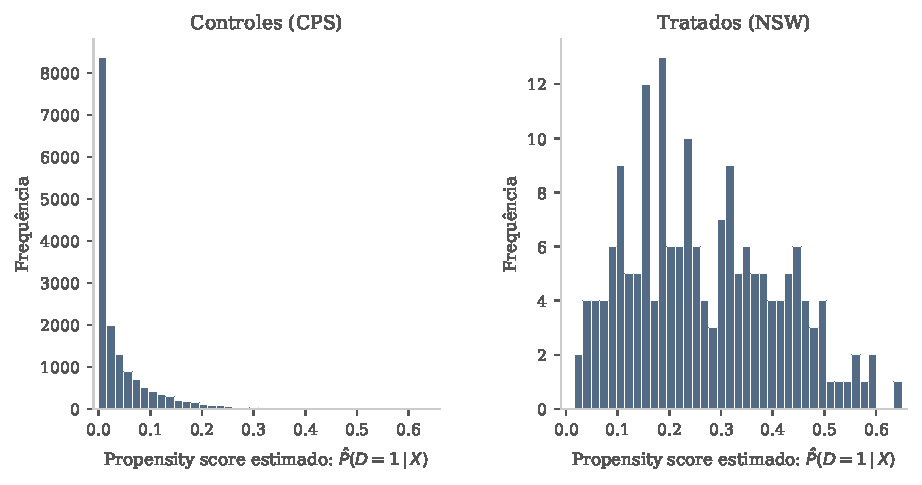
\includegraphics[width=0.9\linewidth]{Figuras/propensity_score.pdf}
    \caption{Distribuição dos \textit{Propensity Scores} estimados para os Controles e Tratados}
    \label{dist}
\end{figure}

\subsubsection{\textit{Nearest-Neighbor} pelo \textit{Propensity Score}}

Uma vez introduzido o \textit{propensity score} como resumo escalar das covariadas, a forma mais natural de usá-lo é simplesmente aplicar nele a mesma lógica de vizinho mais próximo que estudamos antes no caso unidimensional. A ideia é direta: em vez de comparar tratados e controles com base na distância em idade, escolaridade, renda, etc. simultaneamente, passamos a compará-los com base na distância em uma única variável contínua, o $\hat{p}(X_i)$. O problema de pareamento multivariado se transforma, assim, em um problema de pareamento com uma variável só.

No \textit{nearest neighbor} pelo \textit{propensity score}, cada indivíduo tratado é emparelhado com um ou alguns indivíduos de controle cujo \textit{propensity score} seja o mais próximo possível. A noção de “proximidade” aqui é simplesmente a diferença absoluta $|\hat{p}(X_i) - \hat{p}(X_j)|$. Dois indivíduos podem ser muito diferentes em termos de idade e escolaridade, mas se a combinação dessas covariadas leva a uma probabilidade semelhante de tratamento, o método os considera comparáveis do ponto de vista da seleção.

Em termos operacionais, o procedimento pode ser descrito em etapas bastante claras. Primeiro, estima-se o \textit{propensity scor}e $\hat{p}(X_i)$ para toda a amostra. Em seguida, para cada tratado, calcula-se a distância em $\hat{p}(X_i)$ em relação a todos os controles e identifica-se aquele (ou aqueles) que minimizam essa distância. O contrafactual do tratado passa a ser o resultado observado desse(s) controle(s), tal como no vizinho mais próximo com uma variável estudado na Seção 4.

No contexto do NSW, isso significa o seguinte. Em vez de tentar encontrar, para cada participante do programa, um controle que seja simultaneamente parecido em idade, escolaridade, experiência e renda passada, primeiro ajustamos um modelo que explique quem entra ou não entra no programa com base nessas covariadas. Esse modelo nos fornece, para cada indivíduo, uma probabilidade estimada de participação $\hat{p}(X_i)$. Depois, para um jovem tratado com $\hat{p}(X_i) = 0,45$, por exemplo, procuramos no grupo de controle indivíduos cujo $\hat{p}(X_i)$ seja muito próximo de 0,45 — talvez 0,44, 0,46, 0,43. A comparação deixa de ser “quem se parece em todas as características” e passa a ser “quem tinha chances semelhantes de ser selecionado”.

Todas as decisões práticas do pareamento reaparecem aqui, mas agora em um eixo só. Ainda precisamos decidir se vamos usar apenas um controle por tratado ou mais de um. Se optarmos por um único vizinho, o emparelhamento é pontual e muito fácil de interpretar: o tratado é comparado com o controle que tinha probabilidade de tratamento mais parecida com a sua. Se optarmos por dois, três ou mais vizinhos, começamos a construir médias de controles em torno de cada tratado, reduzindo a variância à custa de admitir comparações um pouco menos próximas em $\hat{p}(X_i)$.

Da mesma forma, continua sendo essencial decidir qual é o pior pareamento aceitável. Mesmo em termos de \textit{propensity score}, pode haver tratados em regiões de quase ausência de controles. Por exemplo, indivíduos tratados com $\hat{p}(X_i)$ muito próximo de 1 terão pouquíssimos controles disponíveis na mesma faixa. Na prática, impõe-se um limite máximo para $|\hat{p}(X_i) - \hat{p}(X_j)|$, e tratados que não encontrem controles suficientemente próximos são excluídos da análise. Esse corte explicita a região de suporte comum em termos do \textit{propensity score}: é justamente o intervalo de valores para os quais existem, de fato, tratados e controles.

Em síntese, o \textit{nearest neighbor} pelo \textit{propensity score} combina duas ideias centrais deste capítulo. De um lado, usa o \textit{propensity score} como instrumento de redução de dimensionalidade, transformando um problema de alta dimensão em um problema unidimensional. De outro, aplica nessa dimensão reduzida a lógica já familiar do pareamento por vizinho mais próximo. O resultado é um procedimento que torna viável, na prática, a lógica da CIA em aplicações com muitas covariadas, preservando a transparência da comparação individual entre tratados e controles.

A seguir, iremos estimar tanto o ATE quanto o ATT utilizando vizinhos mais próximo com o \textit{propensity score}. O bloco de código abaixo prepara os dados e estima o propensity score.

\begin{boxH}
\begin{lstlisting}[language = R]

# -----------------------------
# 1) Preparação + estimação do propensity score
# -----------------------------
covs <- c("age", "educ", "black", "hisp", "marr", "nodegree",
          "re74", "re75", "u74", "u75")

vars_needed <- c("treat", "re78", covs)

dat <- cps %>%
  dplyr::select(all_of(vars_needed)) %>%
  tidyr::drop_na() %>%
  mutate(treat = as.integer(treat))

# Logit para propensity score
fml_ps <- as.formula(paste("treat ~", paste(covs, collapse = " + ")))
ps_model <- glm(fml_ps, data = dat, family = binomial("logit"))

dat <- dat %>%
  mutate(pscore = predict(ps_model, type = "response"))

# Vetores para Matching::Match
Y  <- dat$re78
Tr <- dat$treat

# X como matriz N x 1 (propensity score)
Xps <- as.matrix(dat$pscore)

\end{lstlisting}
\end{boxH}

A seguir, iremos construir a função auxiliar \texttt{run\_nn\_ps} para facilitar o cálculo dos resultados.

\begin{boxH}
\begin{lstlisting}[language = R]

# -----------------------------
# 2) Função auxiliar para rodar NN matching no pscore
# -----------------------------
run_nn_ps <- function(M, estimand = c("ATT", "ATE")) {
  estimand <- match.arg(estimand)
  
  out <- Match(
    Y = Y,
    Tr = Tr,
    X = Xps,          # distância é |ps_i - ps_j|
    M = M,
    replace = TRUE,
    estimand = estimand
  )
  
  tibble(
    estimand = estimand,
    M = M,
    estimate = out$est,
    se_AI = out$se,
    t_stat = out$t
  )
}

\end{lstlisting}
\end{boxH}

Por fim, iremos estimar o ATE e o ATT para três valores de vizinhos mais próximos: 1, 3 e 5.

\begin{boxH}
\begin{lstlisting}[language = R]

# -----------------------------
# 3) Rodar M = 1, 3, 5 (ATT e ATE)
# -----------------------------
Ms <- c(1, 3, 5)

results_ps <- bind_rows(
  lapply(Ms, run_nn_ps, estimand = "ATT"),
  lapply(Ms, run_nn_ps, estimand = "ATE")  # remova esta linha se quiser apenas ATT
) %>%
  mutate(est_se = sprintf("%.3f (%.3f)", estimate, se_AI))

print(results_ps)

\end{lstlisting}
\end{boxH}

A Tabela \ref{nnps} apresenta as estimativas obtidas por pareamento de vizinho mais próximo utilizando o \textit{propensity score} como métrica de distância. No Painel A, observa-se que as estimativas do efeito médio sobre os tratados (ATT) são positivas e, em magnitude, mais próximas do efeito estimado a partir dos dados experimentais quando comparadas às estimativas obtidas por métodos ingênuos. Além disso, o ATT mostra relativa estabilidade à escolha do número de vizinhos mais próximos, o que sugere que o \textit{propensity score}, ao resumir a informação das covariadas em uma única dimensão, permite construir um grupo de controle mais comparável aos tratados ao menos nas regiões em que há algum grau de sobreposição. Esses resultados indicam que o pareamento pelo \textit{propensity score} consegue reduzir parte do viés de seleção relevante para a população tratada.

Em contraste, o Painel B evidencia que a estimação do efeito médio do tratamento (ATE) permanece problemática. As estimativas do ATE são negativas, sensíveis à escolha do número de vizinhos mais próximos e distantes do efeito experimental, refletindo a dificuldade de identificar efeitos causais médios em toda a população a partir de dados não experimentais. Como o ATE exige comparações válidas ao longo de toda a distribuição de covariadas, incluindo regiões com baixa probabilidade de tratamento, o pareamento por vizinho mais próximo acaba recorrendo a comparações entre unidades pouco semelhantes, o que introduz extrapolação implícita e viés residual. Assim, mesmo utilizando o \textit{propensity score} como critério de pareamento, o pareamento continua incapaz de recuperar um efeito causal para a população como um todo, ressaltando a importância do suporte comum e os limites do ATE em contextos observacionais.

\begin{table}[htbp]
\centering
\caption{Nearest Neighbor Matching pelo Propensity Score}
\label{tab:nn_pscore_trimmed}
\begin{tabular}{lccc}
\toprule
 & \multicolumn{3}{c}{Número de vizinhos mais próximos ($M$)} \\
\cmidrule(lr){2-4}
 & $1$ & $3$ & $5$ \\
\midrule
\multicolumn{4}{l}{\textbf{Painel A: Efeito Médio sobre os Tratados (ATT)}} \\
\midrule
Tratamento 
& 1322.142 
& 1075.699 
& 1193.554 \\
 
& (943.412) 
& (818.544) 
& (812.322) \\
\midrule
\multicolumn{4}{l}{\textbf{Painel B: Efeito Médio do Tratamento (ATE)}} \\
\midrule
Tratamento 
& -4027.222 
& -7149.183 
& -7009.720 \\
 
& (4238.945) 
& (3389.585) 
& (2771.592) \\
\bottomrule
\end{tabular}

\begin{flushleft}
\footnotesize
\textit{Notas}: A tabela reporta estimativas do efeito médio do tratamento sobre os tratados (ATT) e do efeito médio do tratamento (ATE) obtidas por matching de vizinho mais próximo utilizando o propensity score como métrica de distância. O número de vizinhos mais próximos é indicado por $M$. Os erros-padrão (entre parênteses) seguem a correção analítica de Abadie--Imbens. Todos os pareamentos são realizados com reposição.
\end{flushleft}\label{nnps}
\end{table}


Na subseção seguinte, veremos uma forma alternativa de usar o \textit{propensity score}: em vez de selecionar vizinhos com $\hat{p}(X_i)$ semelhante, vamos utilizar o próprio \textit{propensity score} para construir pesos e formar grupos sintéticos de comparação, por meio de métodos de ponderação.

\subsubsection{Ponderação pelo \textit{Propensity Score}}

Na subseção anterior, utilizamos o \textit{propensity score} para selecionar comparações locais, emparelhando cada tratado com controles de propensão semelhante. Há, porém, uma segunda forma — igualmente natural e muito poderosa — de explorar a propriedade de balanceamento do \textit{propensity score}: em vez de selecionar vizinhos, podemos utilizá-lo diretamente para construir pesos, formando grupos sintéticos de comparação. Essa abordagem é conhecida como ponderação pelo \textit{propensity score}.

A lógica econômica da ponderação é a seguinte. Se indivíduos com diferentes probabilidades de tratamento estão desproporcionalmente representados nos grupos de tratados e controles, podemos reponderar as observações de modo que, após a ponderação, a composição dos grupos se torne comparável. Em vez de “escolher” explicitamente quem será comparado com quem, o método ajusta automaticamente o peso de cada observação para corrigir o viés de seleção observável.

Sob a Hipótese de Independência Condicional, a identificação do efeito causal depende apenas de tornar a seleção no tratamento independente dos resultados potenciais. Como vimos na Seção 5.2, essa independência é garantida ao condicionarmos no \textit{propensity score}. A ponderação faz isso não por meio de condicionamento direto, mas por meio da reconstrução artificial da distribuição das covariadas.

Considere, por exemplo, um indivíduo com probabilidade muito baixa de participar do programa, digamos $\hat{p}(X_i) = 0,1$. Se ele aparece no grupo tratado, esse tipo de indivíduo é “raro” entre os tratados e deve receber peso pequeno. Já no grupo de controle, esse tipo de indivíduo é muito comum e, portanto, deve receber peso elevado. O oposto ocorre para indivíduos com \textit{propensity score} alto. Assim, a ponderação usa exatamente a escassez ou abundância relativa de cada perfil para corrigir o viés de composição.

O resultado desse processo é a construção de uma pseudo-população na qual, por construção, a distribuição das covariadas é a mesma entre tratados e controles. Nessa pseudo-população, a alocação do tratamento é, no sentido observável, tão boa quanto aleatória. O estimador por ponderação mais básico é o chamado \textit{Inverse Probability Weighting} (IPW). Quando o objetivo é identificar o ATE, o estimador ponderado é dado por
$$
\widehat{ATE}_{IPW} = \frac{1}{N} \sum_{i=1}^{N}\left(\frac{D_i Y_i}{\hat{p}(X_i)} - \frac{1- D_iY_i}{1-\hat{p}(X_i)}\right)
$$

A interpretação dessa expressão é direta. Cada resultado observado dos tratados é inflado pelo inverso da sua probabilidade de tratamento, enquanto cada resultado observado dos controles é inflado pelo inverso da sua probabilidade de não tratamento. Observações que eram improváveis de estar no grupo em que de fato estão recebem peso maior.

Quando o objetivo é o Efeito Médio sobre os Tratados (ATT), a ponderação muda apenas no grupo de controle. O estimador passa a ser

$$
\widehat{ATT}_{IPW} = \frac{1}{N_1} \sum_{i : D_i = 1} Y_i - \frac{1}{N_1} \sum_{i : D_i = 0} \frac{\hat{p}(X_i)}{1-\hat{p}(X_i)}Y_i,
$$

\noindent onde $N_1$ é o número de tratados. esse caso, os tratados entram com peso unitário, e os controles são reponderados para reproduzir a distribuição dos tratados em termos de \textit{propensity score.
}
Do ponto de vista conceitual, esse segundo termo corresponde exatamente ao contrafactual médio dos tratados, construído como uma média ponderada dos resultados dos controles, em que os pesos dependem da razão $\frac{\hat{p}(X_i)}{1-\hat{p}(X_i)}$.

Abaixo, iremos estimar o ATE e o ATT através dos estimadores de IPW. No bloco de código a seguir, iremos preparar as variáveis e calcular o \textit{propensity score}.

\begin{boxH}
\begin{lstlisting}[language = R]
# -----------------------------
# 1) Preparação + propensity score
# -----------------------------
covs <- c("age", "educ", "black", "hisp", "marr", "nodegree",
          "re74", "re75", "u74", "u75")

vars_needed <- c("treat", "re78", covs)

dat <- cps %>%
  dplyr::select(all_of(vars_needed)) %>%
  tidyr::drop_na() %>%
  mutate(treat = as.integer(treat))

fml_ps <- as.formula(paste("treat ~", paste(covs, collapse = " + ")))
ps_model <- glm(fml_ps, data = dat, family = binomial("logit"))

dat <- dat %>%
  mutate(pscore = predict(ps_model, type = "response"))

\end{lstlisting}
\end{boxH}

A seguir, iremos limitar nossa amostra para valores do \textit{propensity score} acima de 0,1 e abaixo de 0,9. Isso nos ajuda a evitar pesos extremos, que podem alterar nosso resultado de forma substancial.

\begin{boxH}
\begin{lstlisting}[language = R]
# -----------------------------
# 2) Trimming (recomendado)
# -----------------------------
dat <- dat %>%
  filter(!(pscore >= 0.9)) %>% 
  filter(!(pscore <= 0.1))

\end{lstlisting}
\end{boxH}

No bloco de código abaixo iremos calcular os pesos referentes aos estimadores de IPW do ATE e do ATT.

\begin{boxH}
\begin{lstlisting}[language = R]


# -----------------------------
# 3) IPW weights (ATE e ATT)
# -----------------------------

dat <- dat %>%
  mutate(
    # Pesos brutos
    w_ate = treat/pscore + (1 - treat)/(1 - pscore),
    
    w_att = ifelse(treat == 1, 1, pscore/(1 - pscore))
  ) 

\end{lstlisting}
\end{boxH}

Por fim, iremos estimar o ATE e o ATT usando os pesos construídos no bloco acima.

\begin{boxH}
\begin{lstlisting}[language = R]
# -----------------------------
# 4) Estimativas IPW (ATE e ATT)
# -----------------------------


fit_ate <- lm_robust(re78 ~ treat, data = dat, weights = w_ate)

fit_att <- lm_robust(re78 ~ treat, data = dat, weights = w_att)

summary(fit_ate)
summary(fit_att)

\end{lstlisting}
\end{boxH}

A Tabela \ref{ipw} apresenta as estimativas obtidas por ponderação inversa da probabilidade de tratamento (IPW). Diferentemente dos resultados baseados em regressões simples e em pareamento por vizinho mais próximo, o IPW produz estimativas tanto do efeito médio do tratamento (ATE) quanto do efeito médio sobre os tratados (ATT) que se aproximam substancialmente do efeito estimado a partir dos dados experimentais. Em particular, o ATT estimado é positivo, estatisticamente significativo e de magnitude muito semelhante àquela obtida no experimento, indicando que a reponderação das observações do grupo de controle consegue reproduzir de forma mais adequada o contrafactual relevante para os indivíduos tratados.

Além disso, o IPW também apresenta um desempenho superior na estimação do ATE, cujo valor estimado é positivo e consideravelmente mais próximo do efeito experimental quando comparado às estimativas obtidas por pareamento. Esse resultado sugere que, ao explorar de maneira contínua a informação contida no \textit{propensity score} e utilizar toda a amostra disponível por meio de pesos, o IPW reduz a necessidade de extrapolações extremas implícitas nos métodos de pareamento por vizinhos mais próximos. Ainda que a validade dessas estimativas dependa fortemente da correta especificação do \textit{propensity score} e da existência de suporte comum, os resultados da tabela indicam que a ponderação inversa constitui uma abordagem mais eficaz para recuperar efeitos causais médios em dados não-experimentais, especialmente quando o objetivo é aproximar tanto o ATT quanto o ATE do benchmark experimental.


\begin{table}[h]
\centering
\caption{Resultados do IPW}
\begin{talltblr}[         %% tabularray outer open
entry=none,label=none,
note{}={+ p \num{< 0.1}, * p \num{< 0.05}, ** p \num{< 0.01}, *** p \num{< 0.001}},
]                     %% tabularray outer close
{                     %% tabularray inner open
colspec={Q[]Q[]Q[]},
column{2-3}={}{halign=c,},
column{1}={}{halign=l,},
hline{4}={1-3}{solid, black, 0.05em},
}                     %% tabularray inner close
\toprule
& ATE & ATT \\ \midrule %% TinyTableHeader
Tratamento \hspace{80mm} & \num{1533.798}+ & \num{2056.846}** \\
& (\num{807.560}) & (\num{775.559}) \\
Num.Obs. & \num{452} & \num{452} \\
\bottomrule
\end{talltblr}\label{ipw}
\end{table} 

Um aspecto crucial da ponderação é que ela é particularmente sensível a problemas de suporte comum. Se houver indivíduos com $\hat{p}(X_i)$ muito próximo de 0 ou de 1, os pesos $1/\hat{p}(X_i)$ ou $1/(1-\hat{p}(X_i))$ tornam-se extremamente elevados, fazendo com que poucas observações dominem o estimador. Por esse motivo, na prática, é comum aplicar cortes no \textit{propensity score}, excluindo observações com valores extremos, ou truncar os pesos.

Esse problema é menos agudo no \textit{nearest neighbor}, que simplesmente descarta tratados sem bons controles. Na ponderação, por outro lado, indivíduos mal suportados permanecem na amostra, mas entram com pesos desproporcionalmente grandes, o que pode aumentar drasticamente a variância e gerar instabilidade.

As duas abordagens exploram a mesma base teórica — o \textit{propensity score} como estatística de balanceamento sob a CIA —, mas o fazem de maneiras complementares. O \textit{nearest neighbor} constrói o contrafactual individual de cada tratado por meio de comparações locais. A ponderação constrói o contrafactual médio por meio de uma transformação global da amostra.

No contexto do NSW, isso significa que, em vez de procurar, para cada participante do programa, um controle com probabilidade semelhante de participação, podemos utilizar todos os controles disponíveis, atribuindo pesos maiores àqueles cujo perfil os torne mais parecidos com os tratados em termos de seleção observável. Ambas as estratégias buscam o mesmo objetivo: reproduzir, com dados observacionais, a lógica de um experimento aleatório.

\subsection{Notas sobre Inferência}

Ao longo deste guia, adotamos procedimentos de inferência que refletem a prática empírica padrão para métodos de matching e ponderação, mas é importante deixar explícito que a inferência nesses contextos envolve sutilezas técnicas relevantes. Diferentemente de regressões lineares usuais, os estimadores baseados em matching e em propensity score dependem de objetos estimados em uma primeira etapa, o que altera sua distribuição amostral e torna inadequada a aplicação direta de fórmulas clássicas de variância.

No caso do nearest neighbor matching, a inferência é particularmente delicada devido à não suavidade do estimador e à reutilização de observações do grupo de controle. Por esse motivo, utilizamos a correção analítica proposta por Abadie e Imbens, que ajusta os erros-padrão levando explicitamente em conta a estrutura do pareamento. Essa abordagem constitui a referência padrão na literatura para inferência em matching por vizinho mais próximo.

No caso da ponderação pelo propensity score (IPW), a inferência prática costuma ser realizada por meio de erros-padrão robustos obtidos a partir de regressões ponderadas. Esse procedimento trata o propensity score estimado como conhecido e, portanto, não incorpora explicitamente a incerteza da primeira etapa. Sob condições regulares — como modelos bem especificados e amostras moderadas — essa aproximação tende a funcionar razoavelmente bem e é amplamente utilizada em aplicações empíricas. Ainda assim, ela não é plenamente eficiente do ponto de vista assintótico geral.

A literatura recente tem enfatizado métodos de inferência mais rigorosos baseados em funções de influência e em estimadores doubly robust, como o AIPW e o TMLE, que permitem incorporar automaticamente a incerteza da estimação do propensity score e de modelos auxiliares. Esses métodos representam o estado da arte em inferência causal com dados observacionais, mas exigem ferramentas conceituais e computacionais mais avançadas, que fogem do escopo introdutório deste guia.

Para leitores interessados em aprofundar-se nesses temas, as seguintes referências são particularmente recomendadas:


\begin{itemize}
    \item Abadie e Imbens (2006, 2008), para fundamentos teóricos e inferência em matching por vizinho mais próximo;

\item Hirano, Imbens e Ridder (2003), para resultados assintóticos em estimadores baseados em propensity score;

\item van der Laan e Rose (2011), para inferência via TMLE;

\item Chernozhukov et al. (2018), para estimadores doubly robust com cross-fitting e aprendizado de máquina.
\end{itemize}

Em síntese, os métodos apresentados neste guia fornecem inferência adequada para aplicações empíricas padrão, ao mesmo tempo em que abrem caminho para abordagens mais sofisticadas quando maior rigor inferencial é necessário.
